\documentclass[a4paper,12pt]{article}
\usepackage[utf8]{inputenc}
\usepackage[framed]{mcode}
\usepackage[T1]{fontenc}
\usepackage{listings}
\usepackage{hyperref}
\usepackage{xcolor, graphicx}
\usepackage{float}


\title{Matlab Exercise 3 2018}
\author{Linnéa Olsson & André Frisk}
\date{October 2018}
\begin{document}\maketitle\hrulefill\vs

\maketitle

\section{Abstract}
The main purpose of this exercise is to get a better understanding of heuristic and whats it is. Another goal with this exercise is to learn how to put together two methods of solving that in the end hopefully will provide a better result. In this lab we are supposed to create an AI which works better than the AIs we created before by using old scripts and using parameters as weights. By doing so, we managed to create a AI which gave the best result possible for these simple AIs.                     


\section{Introduction}
In this exercise MATLAB is used to create a bot for the game 2048. the goal of 2048 is to create a tile with the value 2048 by moving all the tiles left, right, up or down on a board measuring four by four tiles. This lab exercise involves us to get to know how the AI works, by using an already existing AI then trying it out and later on put the first AI together with another AI and last but not least design our own AI and compare it to the already existing ones.

\section{Method}
\subsection{Tools/Material}

\begin{itemize}
    \item {\setlength{\parindent}{0cm}
          A computer fitting for the task
          }
    \item $\LaTeX$ editor, in this lab Overleaf was used
    \item MATLAB
    \item EX3\_perspective.zip (\href{https://hh.blackboard.com/bbcswebdav/pid-211496-dt-content-rid-1644399_1/xid-1644399_1}{\color{blue}{link}})
\end{itemize}


\subsection{Implementation}
Except for the file Game2048Simulator.m the following script are used or the lab. The script is mainly used for Task 2.
{\setlength{\parindent}{0cm}
}
\begin{lstlisting}
}function direction = myAI6(A)
B = convertToLogBoard(A);  
d = {'up', 'down', 'right', 'left'};

heuristicValues = zeros(1,4);
for i = 1:length(d)
  Bnew    = slide(B,d{i}); 
  if  isequal(Bnew ,B);             
    heuristicValues(i) = -Inf;
  else
    heuristicValues(i) = ...
      heuristic0(Bnew);
  end
end

[valueMax, iMax] = max(heuristicValues);  
direction = d{iMax};
end

function a = heuristic0(B)
u  =  sum(B(:) == 0);
y  =  - sum(B(:));
a =   sum(1-0.25)*u+(0.25*y);
end

function B =convertToLogBoard(B)
   B(isnan(B)) = 1;
   B = log2(B);
end
\end{lstlisting}


\section{Result}
\subsection{Task 1}
So what happens with AI5? The script for AI5 works that first the script converts every number to logarithms. The scripts run four times before every move in the game because the script predicts which path is the best to choose, left, right, up or down. If nothing of these four predictions works (that no number combines) then the script put the heuristic to be negative infinity. Then the numbers according to the script becomes negative and the script choose the closest path/number to zero. For example if we have [-5, -5, -3, -2] the script will then chose the -2 path as its closest to zero. Also the AI want to have as many zeros as possible, if so the AI works best. When the script have many zeros that means we have a high heuristic value and a low heuristic value if there aren't many zeros. Check the examples below.
\\

Following is the logarithmic identity:
\begin{math}
log_{y}(ab) = log_{y}(a) + log_{y}(b)
\end{math}
\\

The following are two boards with a low heuristic values, the left is the 2048 board and the right is the one with heuristic values:
\begin{center}
\begin{tabular}{| c | c | c | c |}
        \hline
        128 & 64 & 16 & 8  \\
        \hline
        32 & 16 & 16 & 4  \\
        \hline
        4 & 2 & 4 & 2   \\
        \hline
        0 & 2 & 2 & 4\\
        \hline
\end{tabular}
\hspace{0.4cm}
\begin{tabular}{| c | c | c | c |}
        \hline
        7 & 6 & 4 & 3  \\
        \hline
        5 & 4 & 4 & 2  \\
        \hline
        2 & 1 & 2 & 1   \\
        \hline
        0 & 1 & 1 & 2   \\
        \hline
\end{tabular}
\end{center}
\\

\begin{center}
\begin{tabular}{| c | c | c | c |}
        \hline
        8 & 64 & 256 & 8  \\
        \hline
        16 & 16 & 8 & 4  \\
        \hline
        4 & 2 & 32 & 2   \\
        \hline
        0 & 2 & 16 & 4\\
        \hline
\end{tabular}
\hspace{0.4cm}
\begin{tabular}{| c | c | c | c |}
        \hline
        3 & 6 & 8 & 3  \\
        \hline
        4 & 4 & 3 & 2  \\
        \hline
        2 & 1 & 5 & 1   \\
        \hline
        2 & 1 & 4 & 0   \\
        \hline
        
\end{tabular}
\end{center}

The following are two boards with a high heuristic value, the left is the 2048 board and the right is the one with heuristic values:
\begin{center}
\begin{tabular}{| c | c | c | c |}
        \hline
        2 & 0 & 0 & 0  \\
        \hline
        2 & 0 & 0 & 0  \\
        \hline
        0 & 0 & 0 & 2   \\
        \hline
        0 & 0 & 8 & 4\\
        \hline
\end{tabular}
\hspace{0.4cm}
\begin{tabular}{| c | c | c | c |}
        \hline
        1 & 0 & 0 & 0  \\
        \hline
        1 & 0 & 0 & 0  \\
        \hline
        0 & 0 & 0 & 1   \\
        \hline
        0 & 0 & 3 & 2   \\
        \hline
\end{tabular}
\end{center}
\\

\begin{center}
\begin{tabular}{| c | c | c | c |}
        \hline
        0 & 0 & 0 & 2  \\
        \hline
        0 & 0 & 0 & 0  \\
        \hline
        0 & 0 & 0 & 16   \\
        \hline
        2 & 0 & 2 & 32\\
        \hline
\end{tabular}
\hspace{0.4cm}
\begin{tabular}{| c | c | c | c |}
        \hline
        0 & 0 & 0 & 1  \\
        \hline
        0 & 0 & 0 & 0  \\
        \hline
        0 & 0 & 0 & 4   \\
        \hline
        1 & 0 & 1 & 5   \\
        \hline
\end{tabular}
\end{center}


\subsection{Task 2}
The following histograms are the result with a simulation of 300 tries with 2048. The colors indicate the highest tile achieved during the simulations.

\begin{figure}[H]
  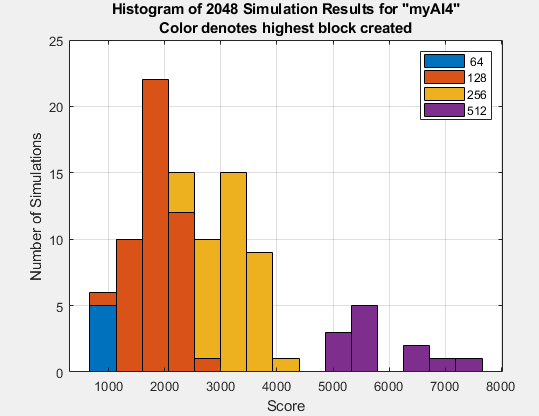
\includegraphics[width=\linewidth]{histogrammyAI4.png}
  \caption{Amount of tries with highest tile achieved}
  \label{fig:historgram}
\end{figure}

\begin{figure}[H]
  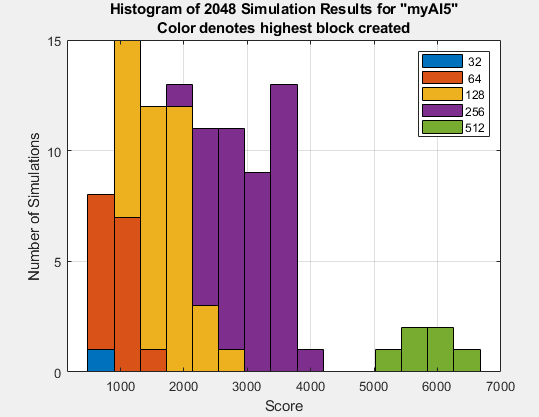
\includegraphics[width=\linewidth]{histogrammyAI5.png}
  \caption{Amount of tries with highest tile achieved}
  \label{fig:historgram}
\end{figure}

\begin{figure}[H]
  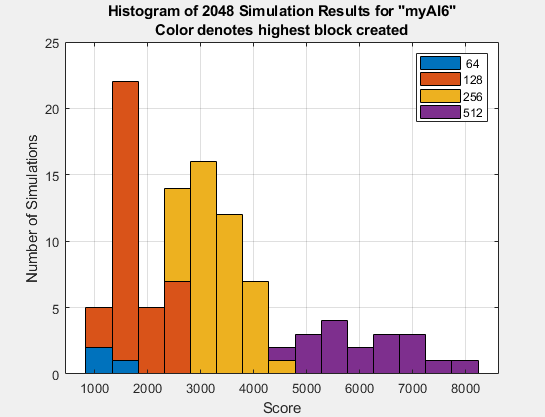
\includegraphics[width=\linewidth]{histogrammyAI6025.png}
  \caption{Amount of tries with highest tile achieved for the weighting 0.25}
  \label{fig:historgram}
\end{figure}

\begin{figure}[H]
  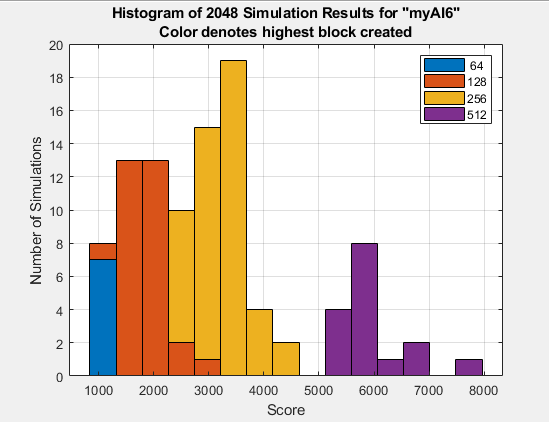
\includegraphics[width=\linewidth]{histogrammyAI6050.png}
  \caption{Amount of tries with highest tile achieved for the weighting 0.50}
  \label{fig:historgram}
\end{figure}

\begin{figure}[H]
  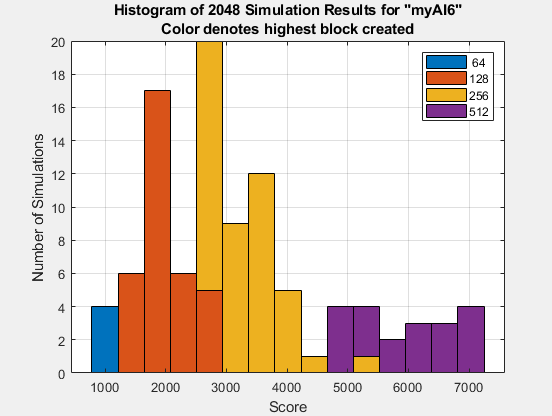
\includegraphics[width=\linewidth]{histogrammyAI6075.png}
  \caption{Amount of tries with highest tile achieved for the weighting 0.75}
  \label{fig:historgram}
\end{figure}




\section{Conclusion}
Task 1's requirements and tasks is responded in result with text, boards and a histogram. The AI5 ain't optional to use to have a AI complete the 2048 game.
\\

In Task 2a the task were to investigate which AI of AI4 and AI5 were the best and in Task 2b were to create a AI6 and investigate with which parameter the AI works better than AI4 and AI5. In Task 2a the AI4 were simply better as it gathered the highest amount of score and the highest amount of the highest tile in this test which was 512.
\\

In Task 2b the parameter used to make AI6 work better than AI4 and AI5 were the weighting  0.75. This is seen because with this parameter the AI gathered the highest amount of tiles of the highest tile that were created with the AI6's three different parameters. The tile 512. There wasn't a big difference between the AI6's different parameters actually. The AI made it to 512 as the highest tile and almost all three parameters gathered estimated 17 512 tiles as its highest in these 300 tries but 0.75 worked the best.



\end{document}